\subsection{Requerimientos y restricciones}

La operatividad del sistema de imitación gestual del robot EVA impone un conjunto de requerimientos funcionales y restricciones paramétricas que delimitan el espacio de soluciones válidas. Dado que el Algoritmo Genético debe converger dentro de la latencia de un solo fotograma de video para garantizar fluidez visual, el presupuesto temporal constituye la restricción primaria del sistema. Adicionalmente, los actuadores mecánicos de silicona poseen límites físicos de operación normalizados: toda tensión calculada debe estar estrictamente acotada al intervalo continuo $[0.0, 1.0]$ para evitar daños estructurales en el elastómero. La codificación binaria, por su parte, impone una resolución discreta que acota la granularidad del control motriz. En la Tabla \ref{TBL_Requerimientos} se sintetizan las restricciones del problema con sus respectivos valores en notación implícita o explícita.

\begin{table}[H]
    \centering
    \footnotesize
    \begin{tabularx}{\textwidth}{|l|X|c|}
        \hline
        \textbf{Restricción} & \textbf{Descripción} & \textbf{Valor / Notación} \\
        \hline
        Tiempo real & Presupuesto máximo de cómputo del AG por cada fotograma capturado & $t_{AG} \leq 33.3$ ms \\
        \hline
        Rango de tensión & Dominio válido de cada variable de decisión $m_i$ & $m_i \in [0.0, 1.0],\ \forall i \in \{1, \dots, 6\}$ \\
        \hline
        Resolución mínima & Sensibilidad de control deseada sobre cada actuador & $\delta = \{x \in \mathbb{R}^+ \mid x \geq 10^{-3}\}$ \\
        \hline
        Espacio de búsqueda & Cardinalidad total del espacio genotípico & $|\mathcal{S}| = 2^{L} = 2^{60}$ combinaciones \\
        \hline
        Resolución de captura & Dimensiones de los fotogramas de entrada & $320 \times 240$ px \\
        \hline
        Convergencia & Umbral de error cuadrático medio aceptable & $E < \epsilon = 0.001$ \\
        \hline
        Diversidad poblacional & Rango saludable de diversidad normalizada de Hamming & $D_{norm} \in [0.2, 0.4]$ \\
        \hline
        Detección facial & Nivel mínimo de confianza de MediaPipe para aceptar un fotograma & Confianza $\geq 0.5$ \\
        \hline
    \end{tabularx}
    \caption{Requerimientos y restricciones del sistema EVA.}
    \label{TBL_Requerimientos}
\end{table}


% ────────────────────────────────────────────────────────────────────────────
%  ANÁLISIS Y DISEÑO
% ────────────────────────────────────────────────────────────────────────────

\subsection{Análisis y Diseño}

% ── Variables de Decisión ──────────────────────────────────────────────────

\subsubsection{Variables de Decisión}
\label{PAR_VariablesDecision}
Se identificaron $n = 6$ variables de decisión que representan la tensión mecánica normalizada de cada actuador del rostro robótico. Cada variable codifica la fracción de contracción de un músculo sintético específico, según se describe en la Tabla \ref{TBL_VariablesDecision}.

\begin{table}[H]
    \centering
    \begin{tabularx}{\textwidth}{|l|l|X|X|}
        \hline
        \textbf{Identificador} & \textbf{Variable de Decisión} & \textbf{Descripción} & \textbf{Efecto} \\
        \hline
        $m_1$ & Tensión mandibular (apertura de boca) & Controla el desplazamiento vertical de la mandíbula inferior del rostro robótico & Cuando $m_1 \to 1.0$, la boca se abre completamente; cuando $m_1 \to 0.0$, permanece cerrada. \\
        \hline
        $m_2$ & Tensión cigomática izquierda (comisura labial izq.) & Controla la elevación o descenso del extremo izquierdo de la boca, determinando la curvatura de la sonrisa en ese lado & Valores altos generan una sonrisa asimétrica izquierda; valores bajos mantienen la comisura neutra o descendente. \\
        \hline
        $m_3$ & Tensión cigomática derecha (comisura labial der.) & Controla la elevación o descenso del extremo derecho de la boca & Equivalente simétrico de $m_2$; la combinación $m_2 \approx m_3 \approx 1.0$ produce una sonrisa bilateral completa. \\
        \hline
        $m_4$ & Tensión orbicular izquierda (párpado izq.) & Controla el grado de apertura o cierre del ojo izquierdo & Cuando $m_4 \to 0.0$, el ojo se cierra (pestañeo); cuando $m_4 \to 1.0$, el ojo está completamente abierto (sorpresa). \\
        \hline
        $m_5$ & Tensión orbicular derecha (párpado der.) & Controla el grado de apertura o cierre del ojo derecho & Equivalente simétrico de $m_4$; la combinación $m_4 \approx m_5 \approx 0.0$ reproduce un doble pestañeo simultáneo. \\
        \hline
        $m_6$ & Tensión frontal (cejas) & Controla la elevación o el fruncimiento de las cejas & Cuando $m_6 \to 1.0$, las cejas se elevan expresando sorpresa; cuando $m_6 \to 0.0$, se fruncen expresando enojo o concentración. \\
        \hline
    \end{tabularx}
    \caption{Variables de decisión}
    \label{TBL_VariablesDecision}
\end{table}

Todas las variables de decisión comparten el dominio continuo $m_i \in [0.0, 1.0]$, donde $0.0$ representa elongación total (músculo completamente relajado) y $1.0$ representa contracción máxima (músculo completamente contraído). Este rango normalizado permite que el sistema sea independiente de las unidades físicas del actuador específico.


% ── Solución o Individuo ──────────────────────────────────────────────────

\subsubsection{Solución o Individuo}

Cada individuo del Algoritmo Genético codifica una configuración completa del rostro robótico como un \textbf{cromosoma binario de $L = 60$ bits}. La estructura de datos empleada es un vector lineal de bits, donde cada segmento consecutivo de $k = 10$ bits representa la tensión de un actuador específico. Esta codificación permite $2^{10} = 1024$ niveles discretos por actuador, logrando una resolución real de $\delta_{real} = \frac{1.0}{1023} \approx 0.000978$.

\begin{figure}[H]
    \centering
    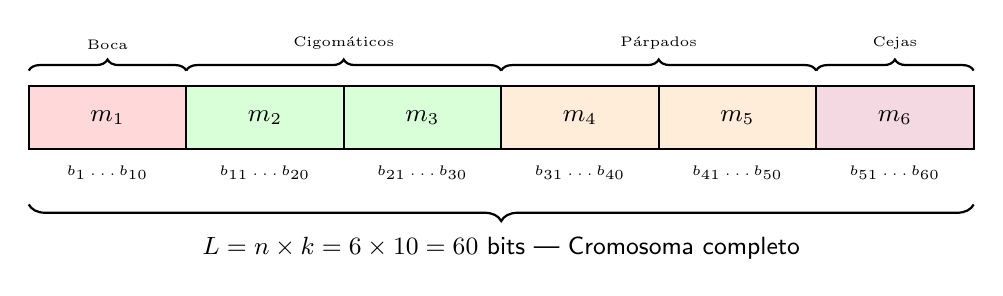
\begin{tikzpicture}[font=\sffamily\small]
        % Segmentos del cromosoma
        \draw[thick, fill=red!15] (0,0) rectangle (2,0.8);
        \node at (1,0.4) {$m_1$};
        \node[font=\tiny] at (1,-0.3) {$b_1 \dots b_{10}$};

        \draw[thick, fill=green!15] (2,0) rectangle (4,0.8);
        \node at (3,0.4) {$m_2$};
        \node[font=\tiny] at (3,-0.3) {$b_{11} \dots b_{20}$};

        \draw[thick, fill=green!15] (4,0) rectangle (6,0.8);
        \node at (5,0.4) {$m_3$};
        \node[font=\tiny] at (5,-0.3) {$b_{21} \dots b_{30}$};

        \draw[thick, fill=orange!15] (6,0) rectangle (8,0.8);
        \node at (7,0.4) {$m_4$};
        \node[font=\tiny] at (7,-0.3) {$b_{31} \dots b_{40}$};

        \draw[thick, fill=orange!15] (8,0) rectangle (10,0.8);
        \node at (9,0.4) {$m_5$};
        \node[font=\tiny] at (9,-0.3) {$b_{41} \dots b_{50}$};

        \draw[thick, fill=purple!15] (10,0) rectangle (12,0.8);
        \node at (11,0.4) {$m_6$};
        \node[font=\tiny] at (11,-0.3) {$b_{51} \dots b_{60}$};

        % Llave inferior
        \draw[decorate, decoration={brace, amplitude=6pt, mirror}, thick]
            (0,-0.7) -- (12,-0.7)
            node[midway, below=8pt] {$L = n \times k = 6 \times 10 = 60$ bits — Cromosoma completo};

        % Etiquetas por grupo muscular
        \draw[decorate, decoration={brace, amplitude=4pt}, thick]
            (0,1.0) -- (2,1.0) node[midway, above=4pt, font=\tiny] {Boca};
        \draw[decorate, decoration={brace, amplitude=4pt}, thick]
            (2,1.0) -- (6,1.0) node[midway, above=4pt, font=\tiny] {Cigomáticos};
        \draw[decorate, decoration={brace, amplitude=4pt}, thick]
            (6,1.0) -- (10,1.0) node[midway, above=4pt, font=\tiny] {Párpados};
        \draw[decorate, decoration={brace, amplitude=4pt}, thick]
            (10,1.0) -- (12,1.0) node[midway, above=4pt, font=\tiny] {Cejas};
    \end{tikzpicture}
    \caption{Estructura del cromosoma binario del individuo. Cada segmento de 10 bits codifica la tensión normalizada de un actuador facial.}
    \label{FIG_Cromosoma}
\end{figure}

La \textbf{decodificación} del segmento de bits del actuador $i$ al valor real $m_i$ se realiza en dos pasos:
\begin{enumerate}
    \item Conversión del segmento binario a valor decimal: $d_i = \sum_{j=0}^{k-1} b_j \cdot 2^{k-1-j}$
    \item Mapeo al rango real: $m_i = a + d_i \cdot \frac{b - a}{2^k - 1} = 0.0 + d_i \cdot \frac{1.0}{1023}$
\end{enumerate}

\textbf{Restricciones sobre el individuo:}
\begin{itemize}
    \item Cada gen decodificado debe satisfacer $m_i \in [0.0, 1.0],\ \forall i \in \{1, \dots, 6\}$. La codificación binaria garantiza esto por construcción.
    \item No existen restricciones de dependencia entre actuadores: cada $m_i$ es independiente, lo que significa que toda combinación de tensiones constituye una configuración válida del sistema.
    \item El tamaño del cromosoma es fijo ($L = n \times k = 60$ bits) y no varía durante la ejecución.
\end{itemize}


% ── Variables a Optimizar ─────────────────────────────────────────────────

\subsubsection{Variables a optimizar}
\label{PAR_VariablesOptimizar}
Con base en las variables de decisión mencionadas en el apartado \ref{PAR_VariablesDecision}, se definieron $m = 5$ variables a optimizar que cuantifican el rendimiento del sistema, según se describen en la Tabla \ref{TBL_VariablesOptimizar}.

\begin{table}[H]
    \centering
    \begin{tabularx}{\textwidth}{|l|l|X|X|}
        \hline
        \textbf{Identificador} & \textbf{Variable a Optimizar} & \textbf{Descripción} & \textbf{Variables de decisión involucradas} \\
        \hline
        $E$ & Error de imitación facial (MSE) & Se determina calculando la distancia cuadrática media entre el vector objetivo $T$ (expresión del usuario humano) y el vector de tensiones $M$ del mejor individuo & Para su cálculo se utilizan todas las variables $m_1, \dots, m_6$ comparadas con sus correspondientes valores objetivo $t_1, \dots, t_6$ extraídos por MediaPipe. \\
        \hline
        $F$ & Aptitud de convergencia (Fitness) & Transformación inversa del error que el AG maximiza para guiar la selección evolutiva & Se calcula directamente a partir de $E$, que a su vez depende de $m_1, \dots, m_6$. \\
        \hline
        $V$ & Velocidad de convergencia generacional & Número de generaciones requeridas por el AG para alcanzar un umbral de error aceptable $E < \epsilon$ ante una expresión facial nueva & Depende indirectamente de la distribución inicial de $m_1, \dots, m_6$ en la población y de los hiperparámetros $p_c$, $p_m$. \\
        \hline
        $S$ & Estabilidad inter-fotograma & Mide la variación promedio del vector $[m_1, \dots, m_6]$ del mejor individuo entre fotogramas consecutivos de video & Compara los valores de $m_1, \dots, m_6$ del mejor individuo entre los fotogramas $f$ y $f-1$. \\
        \hline
        $D$ & Diversidad poblacional & Dispersión genética de la población medida por la distancia de Hamming promedio entre todos los pares de cromosomas & Evalúa la representación binaria de todas las variables $m_1, \dots, m_6$ de todos los individuos de la generación actual. \\
        \hline
    \end{tabularx}
    \caption{Variables a optimizar}
    \label{TBL_VariablesOptimizar}
\end{table}

El \textbf{error de imitación facial} ($E$) se calcula a través de la Ecuación \ref{EQ_VariableOptimizarError}.

\begin{equation}
    E(M, T) = \frac{1}{n} \sum_{i=1}^{n} (t_i - m_i)^2
    \label{EQ_VariableOptimizarError}
\end{equation}

Donde $n = 6$ es el número de actuadores, $t_i$ es el valor objetivo del actuador $i$ extraído por MediaPipe y $m_i$ es la tensión decodificada del cromosoma del individuo. Un valor de $E = 0$ indica imitación perfecta; $E_{max} = 1.0$ cuando todos los actuadores están en el extremo opuesto al objetivo.

Se busca que el $E$ sea \textbf{minimizado}.

La \textbf{aptitud de convergencia} ($F$) se calcula a través de la Ecuación \ref{EQ_VariableOptimizarFitness}.

\begin{equation}
    F(M, T) = \frac{1}{1 + E(M, T)}
    \label{EQ_VariableOptimizarFitness}
\end{equation}

Donde $E$ es el error de imitación. Cuando $E \to 0$, entonces $F \to 1$ (aptitud máxima). Cuando $E$ es grande, $F \to 0$.

Se busca que $F$ sea \textbf{maximizado}.

La \textbf{estabilidad inter-fotograma} ($S$) se calcula a través de la Ecuación \ref{EQ_VariableOptimizarEstabilidad}.

\begin{equation}
    S^{(f)} = \frac{1}{n} \sum_{i=1}^{n} \left( m_i^{(f)} - m_i^{(f-1)} \right)^2
    \label{EQ_VariableOptimizarEstabilidad}
\end{equation}

Donde $m_i^{(f)}$ es la tensión del actuador $i$ del mejor individuo en el fotograma $f$ y $m_i^{(f-1)}$ es la tensión del mismo actuador en el fotograma anterior. Valores de $S > 0.2$ indican movimientos espasmódicos indeseados en el avatar robótico.

Se busca que $S$ sea \textbf{minimizado}.

La \textbf{diversidad poblacional} ($D$) se calcula a través de la Ecuación \ref{EQ_VariableOptimizarDiversidad}.

\begin{equation}
    D^{(g)} = \frac{2}{N(N-1)} \sum_{i=1}^{N-1} \sum_{j=i+1}^{N} d_H(I_i, I_j)
    \label{EQ_VariableOptimizarDiversidad}
\end{equation}

Donde $d_H(I_i, I_j)$ es la distancia de Hamming entre los cromosomas de los individuos $I_i$ e $I_j$ (número de bits en los que difieren). La diversidad normalizada se obtiene como $D_{norm} = D / L$.

Se busca que $D_{norm}$ sea \textbf{equilibrado} dentro del rango $[0.2, 0.4]$: diversidad demasiado baja provoca convergencia prematura (mínimos locales), diversidad demasiado alta impide convergencia (expresión inestable).


% ── Objetivos de Optimización ─────────────────────────────────────────────

\subsubsection{Objetivos de Optimización}
Como resumen de las variables de optimización, mencionadas en el apartado \ref{PAR_VariablesOptimizar}, se presenta la Tabla \ref{TBL_ObjetivosOptimizacion}.

\begin{table}[H]
    \centering
    \begin{tabularx}{\textwidth}{|c|c|X|X|}
        \hline
        \textbf{Identificador} & \textbf{Fórmula} & \textbf{Objetivo de Optimización} & \textbf{Valores} \\
        \hline
        $E$ & Ec. \ref{EQ_VariableOptimizarError} & Minimizar & $E \in [0, 1]$;\ $E = 0$ imitación perfecta \\
        \hline
        $F$ & Ec. \ref{EQ_VariableOptimizarFitness} & Maximizar & $F \in (0, 1]$;\ $F = 1$ aptitud máxima \\
        \hline
        $V$ & Generaciones hasta $E < \epsilon$ & Minimizar & $V \in \{1, 2, \dots, G_{max}\}$ \\
        \hline
        $S$ & Ec. \ref{EQ_VariableOptimizarEstabilidad} & Minimizar & $S \geq 0$;\ $S < 0.05$ transición suave \\
        \hline
        $D$ & Ec. \ref{EQ_VariableOptimizarDiversidad} & Equilibrar & $D_{norm} \in [0.2, 0.4]$ rango saludable \\
        \hline
    \end{tabularx}
    \caption{Variables y objetivos de optimización.}
    \label{TBL_ObjetivosOptimizacion}
\end{table}


% ────────────────────────────────────────────────────────────────────────────
%  BASE DE CONOCIMIENTOS
% ────────────────────────────────────────────────────────────────────────────

\subsection{Base de conocimientos}
El sistema diseñado usa una base de conocimiento implementada como un conjunto de tablas estáticas dentro de un archivo SQLite (\texttt{eva\_conocimiento.db}) que se utiliza para definir el modelo del robot, aplicar las reglas de transformación cinemática y para encontrar el valor de las variables de optimización. Estas tablas son pobladas una única vez antes de iniciar la ejecución y permanecen en modo solo-lectura durante toda la sesión del AG, garantizando que el algoritmo nunca altere las reglas del problema que intenta resolver.

\begin{itemize}
    \item \textbf{Modelo del robot} (\texttt{robot\_modelo}): Es una tabla de datos donde cada fila define un actuador del rostro robótico. Las columnas enlistan los atributos: identificador del actuador ($m_1, \dots, m_6$), nombre biomecánico, rol funcional, número de bits por gen ($k = 10$) y los límites de tensión $[0.0, 1.0]$. Determina la dimensión del cromosoma utilizado por el AG.
    \item \textbf{Mapeo cinemático} (\texttt{mapeo\_cinematico}): Conjunto de reglas de transformación que describen cómo cada combinación de tensiones de los actuadores desplaza visualmente los puntos clave del rostro en el gemelo digital (Pygame). Por ejemplo: si $m_2 = 1.0$ y $m_3 = 1.0$, ambas comisuras labiales ascienden y el sistema renderiza una sonrisa completa.
    \item \textbf{Expresiones de referencia Ekman} (\texttt{expresiones\_ekman}): Catálogo de 6 vectores de tensión ideales $[m_1, \dots, m_6]$ correspondientes a las emociones básicas universales (alegría, tristeza, sorpresa, miedo, enojo y asco), según la taxonomía de Paul Ekman. Se utilizan como referencia de calibración y para validación cruzada.
    \item \textbf{Parámetros biomecánicos del material} (\texttt{parametros\_material}): Constantes que modelan las propiedades físicas del elastómero simulado, como el coeficiente de elasticidad y los límites de deformación, que escalan la señal de los actuadores hacia el movimiento de píxeles en pantalla.
    \item \textbf{Configuración del AG} (\texttt{config\_ag}): Valores por defecto del sistema genético, como tamaño de población ($N$), probabilidad de cruza ($p_c$), probabilidad de mutación ($p_m$), máximo de generaciones ($G_{max}$), umbral de error ($\epsilon$), tamaño del torneo ($k_t$) y número de élites ($e$). Definidos por el usuario antes de la ejecución como punto de partida controlable del experimento.
\end{itemize}

Esta separación arquitectural garantiza que modificar el modelo del robot ---por ejemplo, escalar de 6 a 12 actuadores--- requiera únicamente alterar filas en la tabla \texttt{robot\_modelo}, sin modificar una sola línea del algoritmo genético.


% ────────────────────────────────────────────────────────────────────────────
%  FUNCIÓN DE APTITUD
% ────────────────────────────────────────────────────────────────────────────

\subsection{Función de Aptitud}
Tomando como referencia la Tabla \ref{TBL_ObjetivosOptimizacion}, las soluciones generadas por el Algoritmo Genético se evalúan con el objetivo de identificar cuál es mejor en términos de fidelidad gestual, con este fin se diseñó la función de aptitud (Ecuación \ref{EQ_FuncionAptitud}).

\begin{equation}
    Aptitud(Individuo) = \frac{1}{1 + E(M_{Individuo},\ T)}
    \label{EQ_FuncionAptitud}
\end{equation}

Dado que el $E$ (Error de imitación) es una variable a minimizar, se debe tomar en cuenta que entre más grande sea, la solución codificada en el individuo es menos buena por lo que se propone que pase dividiendo, pero dado que el valor mínimo del error es $E = 0$ (imitación perfecta), se le agrega un $1$ para evitar divisiones por $0$. De este modo:

\begin{itemize}
    \item Cuando $E = 0$ (imitación perfecta): $Aptitud = \frac{1}{1+0} = 1.0$ (aptitud máxima).
    \item Cuando $E \to \infty$ (error enorme): $Aptitud \to 0$ (aptitud nula).
    \item La función es monótonamente decreciente respecto a $E$: a menor error, mayor aptitud.
\end{itemize}

Esta transformación hiperbólica garantiza que $Aptitud \in (0, 1]$ para todo individuo válido, proporcionando al mecanismo de selección por torneo un criterio de comparación estrictamente positivo y acotado superiormente.

\clearpage
